\documentclass[a4paper, twocolumn]{article}
\usepackage[pdftex, hidelinks,
            pdftitle={Machine Learning Report},
            pdfauthor={Erik Sven Vasconcelos Jansson},
            pdfsubject={Machine Learning Report},
            pdfkeywords={report}]{hyperref}

\usepackage{bm}
\usepackage{xcolor}
\usepackage[T1]{fontenc}
\usepackage[utf8]{inputenc}
\usepackage{algorithmic}
\usepackage{algorithm}
\usepackage{amsfonts}
\usepackage{booktabs}
\usepackage{amssymb}
\usepackage{amsthm}
\usepackage{courier}
\usepackage{booktabs}
\usepackage{graphicx}
\usepackage{listings}
\usepackage{mathtools}
\usepackage[capitalize, noabbrev]{cleveref}
\lstset{basicstyle=\footnotesize\ttfamily,
        breakatwhitespace = false,
        breaklines = true,
        keepspaces = true,
        language = R,
        showspaces = false,
        showstringspaces = false,
        belowcaptionskip = \bigskipamount,
        framerule = 0.80pt,
        frame = tb,
        numbers = left,
        belowskip = \bigskipamount,
        escapeinside={<@}{@>}}

\title{Introduction to Machine Learning \\
       Individual Laboration Report --6--}
\author{{Erik Sven Vasconcelos Jansson} \\
        {\href{mailto:erija578@student.liu.se}
        {\texttt{erija578@student.liu.se}}} \\
        {Linköping University, \, Sweden}}
        \newtheorem{theorem}{Theorem}

\begin{document}

    \pagenumbering{arabic}
    \maketitle % Titles...

    Finally, the last machine learning topic covered are \emph{artificial neural networks}. These estimators are very flexible, such that even a \emph{single layer} \emph{feed-forward neural network} complies with the \emph{universal approximation theorem}, presented by \emph{Cs\'aji}~\cite{csaji2001approximation}:

    \begin{theorem}[Universal Approximation Theorem] \label{thm:uat}
        Any artificial feed-forward neural network with a single hidden layer, containing a finite amount of neurons, can approximate any continuous functions on the compact subset $\mathcal{R}^n$ (with restrictions on $\sigma$).
    \end{theorem}

    \begin{proof}
        \emph{Cs\'aji's}~\cite{csaji2001approximation} derivation of Theorem~\ref{thm:uat}.
    \end{proof}

    Basically, the theorem states that even simple neural networks can represent interesting functions, given some suitable subset of \emph{activation functions}. For this assignment, we want to approximate $\sin x$, where we are given \emph{25 observation} for \emph{training set}. Also, we are given a \emph{validation set} of length \emph{25} for checking if our neural network is under/overfitting. We are using the \emph{R package} \verb|neuralnet| for our fit with \emph{10 hidden units} in a \emph{single hidden layer}, also initialized with \emph{random weights} in $[-1, 1]$ interval. See Listing~\ref{lst:neuralnet} for the entire assignment source code.

    For the curious, Equations~\ref{eq:sigmoid}, \ref{eq:batch_gradient}, and \ref{eq:perceptron} are given:

    \begin{equation} \label{eq:sigmoid}
        \sigma(u) = \frac{1}{1 + e^{-u}}
    \end{equation}

    \begin{equation} \label{eq:batch_gradient}
        \bm{w}_{(i)} = \bm{w}_{(i-1)} - \eta_k \nabla E(\bm{w}_{(i-1)})
    \end{equation}

    \begin{equation} \label{eq:perceptron}
        \hat{y}_j(\bm{x}) = \sigma(w_0 + \sum_{h=1}^{H} \sigma(w_{0h} + \bm{w}_h^\intercal\bm{x}))
    \end{equation}

    \newpage
    \begin{enumerate}
        \item{\textbf{Sigmoid Activation Function:} ``S''-shaped function which converges $\sigma(u) = 1$ as $u \to \infty$ and $\sigma(u) = 0$ as $u \to -\infty$. Used in Equation~\ref{eq:perceptron}.}
        \item{\textbf{Batch Gradient Descent:} finds the ``step'' in the right direction for \emph{minimizing error} $E$. This is achieved with the \emph{gradient} of $E$ given in respect to the weights $\bm{w}$; giving a \emph{hyperplane}.}
        \item{\textbf{Single-Layer Neural Network Estimator:} uses Equations~\ref{eq:sigmoid} and \ref{eq:batch_gradient} to find $\hat{y}_j$ by finding the parameters $\bm{w}$ in each layer (a linear equation) by means of \emph{gradient descent} and producing a \emph{non-linear result in subsequent layers} by the \emph{activation function}. This is the primary reason why neural networks are so flexible \& general.}
    \end{enumerate}

    By using a \emph{threshold} for the \emph{gradient descent} we can stop the \emph{neural network} from either \emph{overfitting} or \emph{underfitting}. This simply done by increasing the threshold iteratively and taking the validation set's:

    \begin{table}[h!]
        \begin{center}
            \begin{tabular}{cc}
                \toprule
                \textbf{Threshold} & \textbf{S.S.E.} \\
                \midrule
                0.001 & 0.01367691527 \\
                0.002 & 0.01262419958 \\
                0.003 & 0.00988418900 \\
                0.004 & 0.00850089424 \\
                0.005 & 0.00955545744 \\
                0.006 & 0.00974372099 \\
                0.007 & 0.01583926857 \\
                0.008 & 0.01649252416 \\
                0.009 & 0.02112490377 \\
                0.010 & 0.02735909554 \\
                \bottomrule
            \end{tabular}
        \end{center}
        \caption{Neural Network Values}
        \label{tab:forecast}
    \end{table}

    After finding the ``optimal threshold'' of \emph{0.004} by picking the $4^{th}$ iteration (where $i = 4$ that is) which gives the least amount of error for a validation set, we plot the best neural network in Figure~\ref{fig:network}, and also the predictions in Figure~\ref{fig:predictions} for a \emph{sine function}. Notice that the fit is pretty good, and the estimator gives a pretty ``spot on'' prediction for the function. It seems \emph{neural networks} are incredibly powerful, but take time to train and are harder to reason about (for example, how do we choose the number of hidden layers and units? How long will it take?)

    \nocite{*}
    \bibliographystyle{alpha}
    \bibliography{report}
    \newpage

    \begin{figure}[h!]
        \centering
        \caption{Neural Network}
        \label{fig:network}
        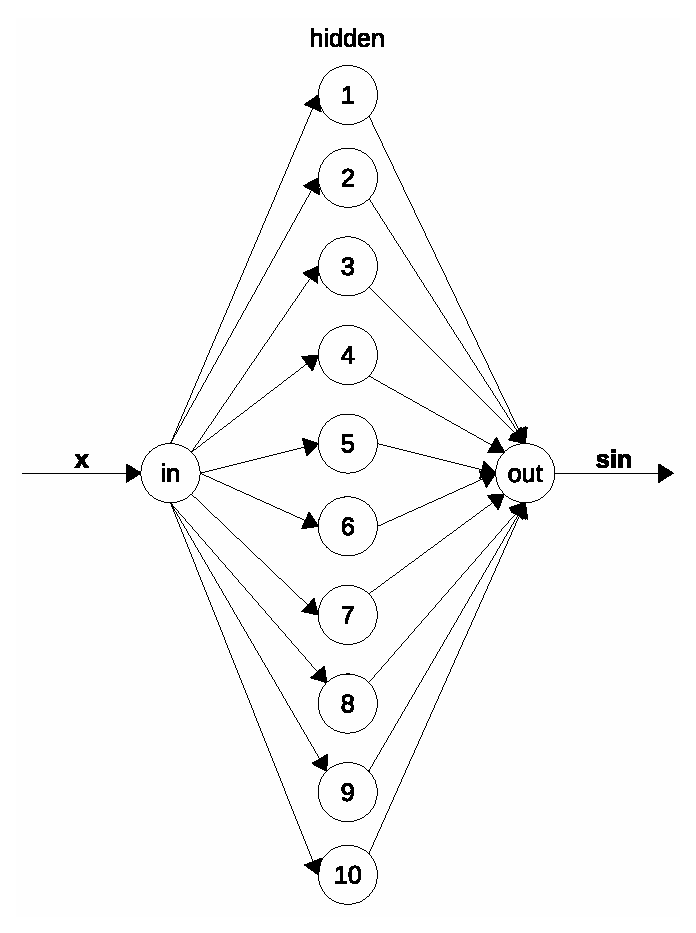
\includegraphics[width=0.46\textwidth]{share/network.eps}
    \end{figure}

    \begin{figure}[h!]
        \centering
        \caption{Neural Network's Produced Predictions (in the graph are \textcolor{blue}{raw values} and \textcolor{red}{predicted values}).}
        \label{fig:predictions}
        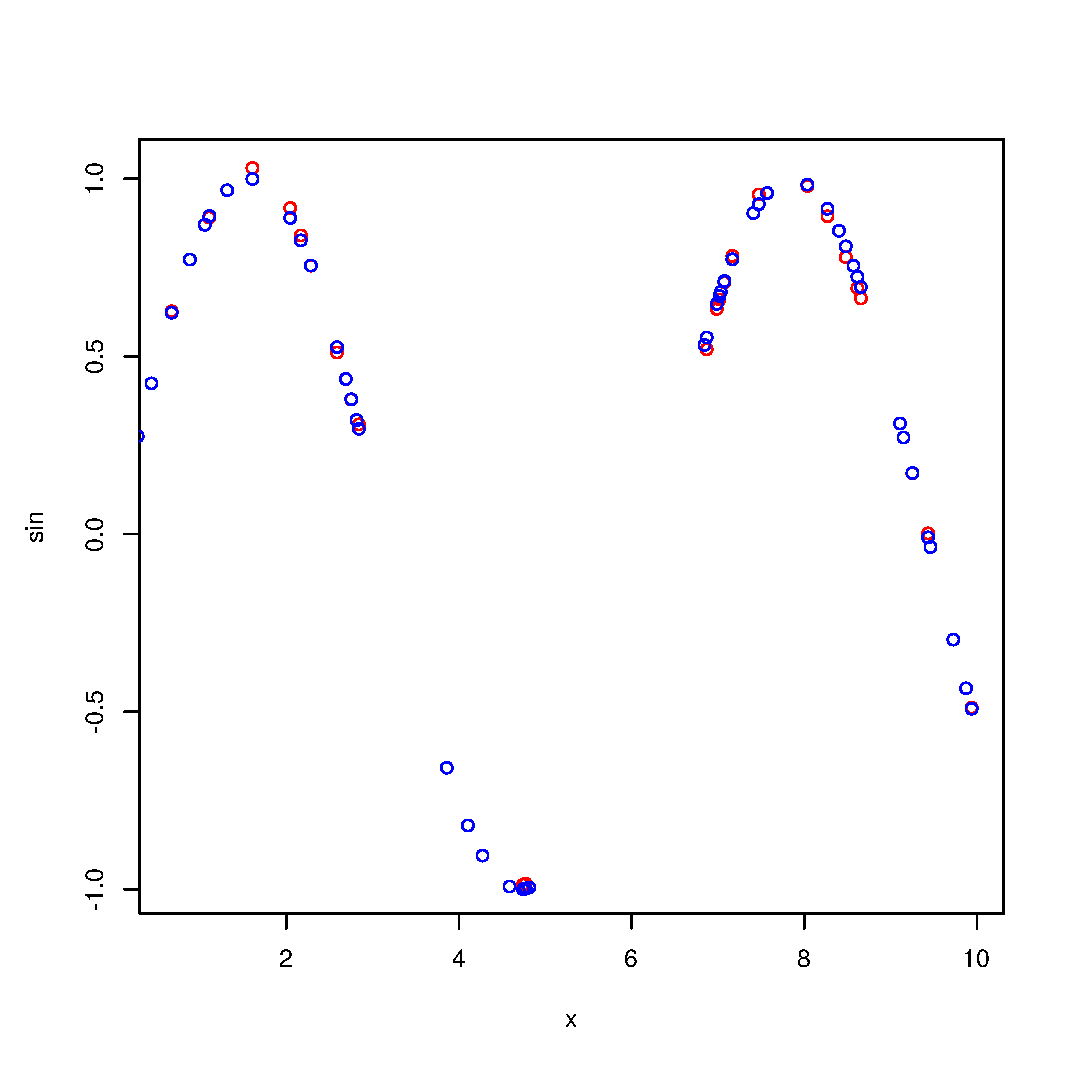
\includegraphics[width=0.5\textwidth]{share/predictions.eps}
    \end{figure}

    \onecolumn \appendix
    \section*{Appendix}

    \lstinputlisting[caption={Feed-Forward Backpropagating Neural Network Sine Estimator Script}, label={lst:neuralnet}]{share/neuralnet.r}
    \lstinputlisting[caption={Output About the Produced Neural Network in the Assignment}, label={lst:properties}]{share/output.txt}

\end{document}
